\newpage
\section{Входные и выходные данные}
\setcounter{figure}{0}

\subsection{Входные данные}
Для осуществления сбора показаний ССД необходимо получить из центральной базы данных список подконтрольных ему УСПД. Так же на ССД должны находиться данные для идентификации и аутентификации на УСПД. 

Списком УСПД является набор строк, которые содержат в себе идентификатор УСПД и его IP-адрес, по которому он доступен в сети интернет.

Список УСПД хранится в базе данных центрального сервера. ССД запрашивает список с ЦС и сохраняет его во временной базе данных. Опрос происходит по списку, сохраненному во временную базу данных. Список из временной базы данных синхронизируется с базой данных центрального сервера через определенные промежутки времени, заданные администратором системы либо по команде от ЦС.

Данными для идентификации и аутентификации являются закрытые ключи шифрования и пары ``имя пользователя'' и ``пароль''.

%TODO имхо маловато для описаия входных данных. добавить формат хотя бы для списка УСПД.

\subsection{Выходные данные}

По запросу ССД получает от УСПД пакет данных который содержит показания УУ, информацию о состоянии УУ и информацию о состоянии УСПД. Структура данного покета представлена на рисунке \ref{img:answer_struct}.

\begin{figure}[!ht]
 \center{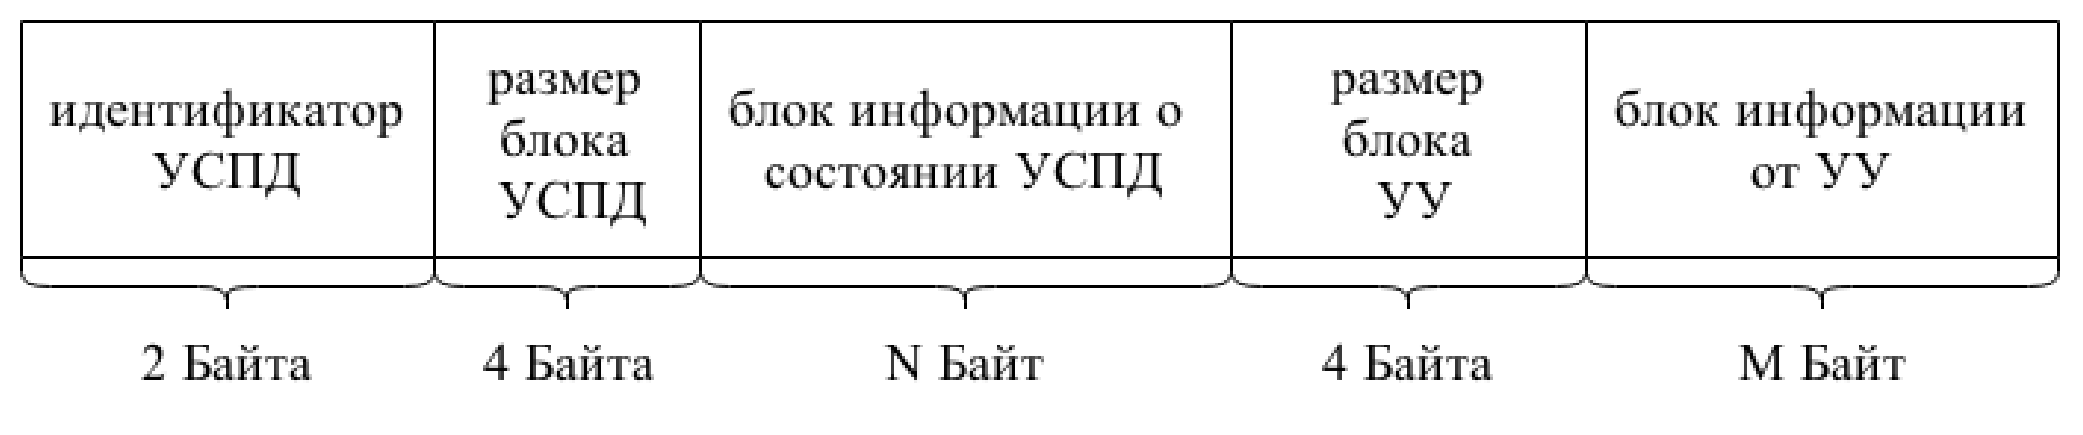
\includegraphics[width=0.8\linewidth]{answer_struct}}
 \caption{Структура пакета, получаемого от УСПД}
 \label{img:answer_struct}
\end{figure}

\newpage
Пакет состоит из пяти блоков:

\begin{enumerate}
 \item идентификатор УСПД - уникальная для каждого УСПД последовательность из 2 байт, позволяющая однозначно идентифицировать УСПД;
 \item размер блока УСПД - размер в байтах блока данных о УСПД (4 байта);
 \item блок информации о состоянии УСПД - информация о состоянии УСПД, текущее времени на УСПД;
 \item блок данных УУ - размер в байтах блока данных о УУ (4 байта);
 \item блок информации от УУ - последовательность структур данных, содержащих информацию о каждом УУ, подконтрольном УСПД и показания данного УУ.
\end{enumerate}

Структура данных, содержащая информацию о каждом УУ представлена на рисунке \ref{img:UU_struct}.

\begin{figure}[!ht]
 \center{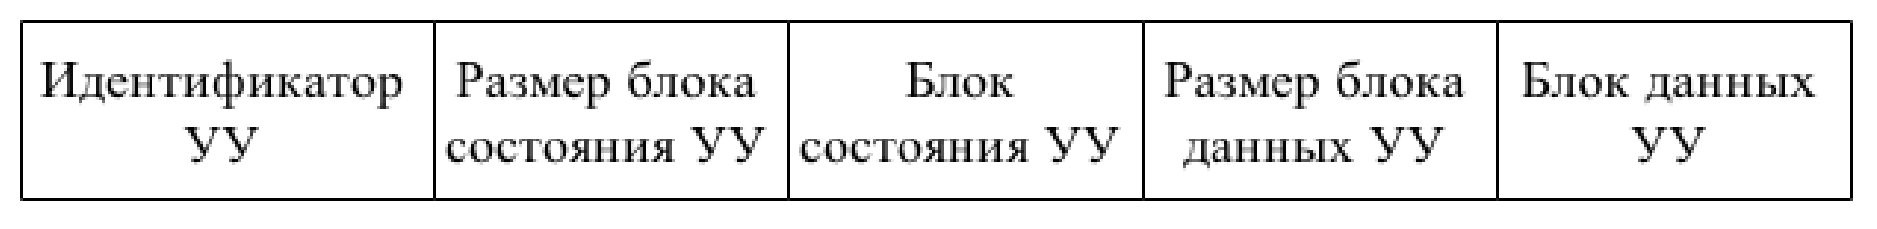
\includegraphics[width=0.8\linewidth]{UU_struct}}
 \caption{Структура данных, получаемая от УУ}
 \label{img:UU_struct}
\end{figure}

Структура состоит из пяти блоков:

\begin{itemize}
 \item идентификатор УУ - уникальный для каждого УУ байт, позволяющий однозначно идентифицировать УУ подконтрольный указанному УСПД;
 \item размер блока состояния УУ - размер в байтах блока информации о состоянии УУ;
 \item блок состояния УУ - блок данных о состоянии УУ;
 \item размер блока данных УУ - размер в байтах блока данных, собранных УУ;
 \item блок данных УУ - данные, собранные прибором учета.
\end{itemize}

Опрос УСПД производится через заданные администратором системы интервалы времени. После получения ответа от УСПД пакет записывается во временную базу данных и начинается его обработка, в процессе которой проверяется структура пакета и преобразование данных в формат, необходимый серверу сбора данных.

На данном этапе проверяется работоспособность УСПД. Контролируетя присутствие ответа на запрос, проверяется содержимой блока состояния УСПД на придмет ошибок работы устройства, проверяется структура данных с показаниями от устройств учета.